%\documentclass{article}
%\usepackage{graphicx,subfigure}
%\begin{document}

\begin{figure}[!h]
  \centering
% 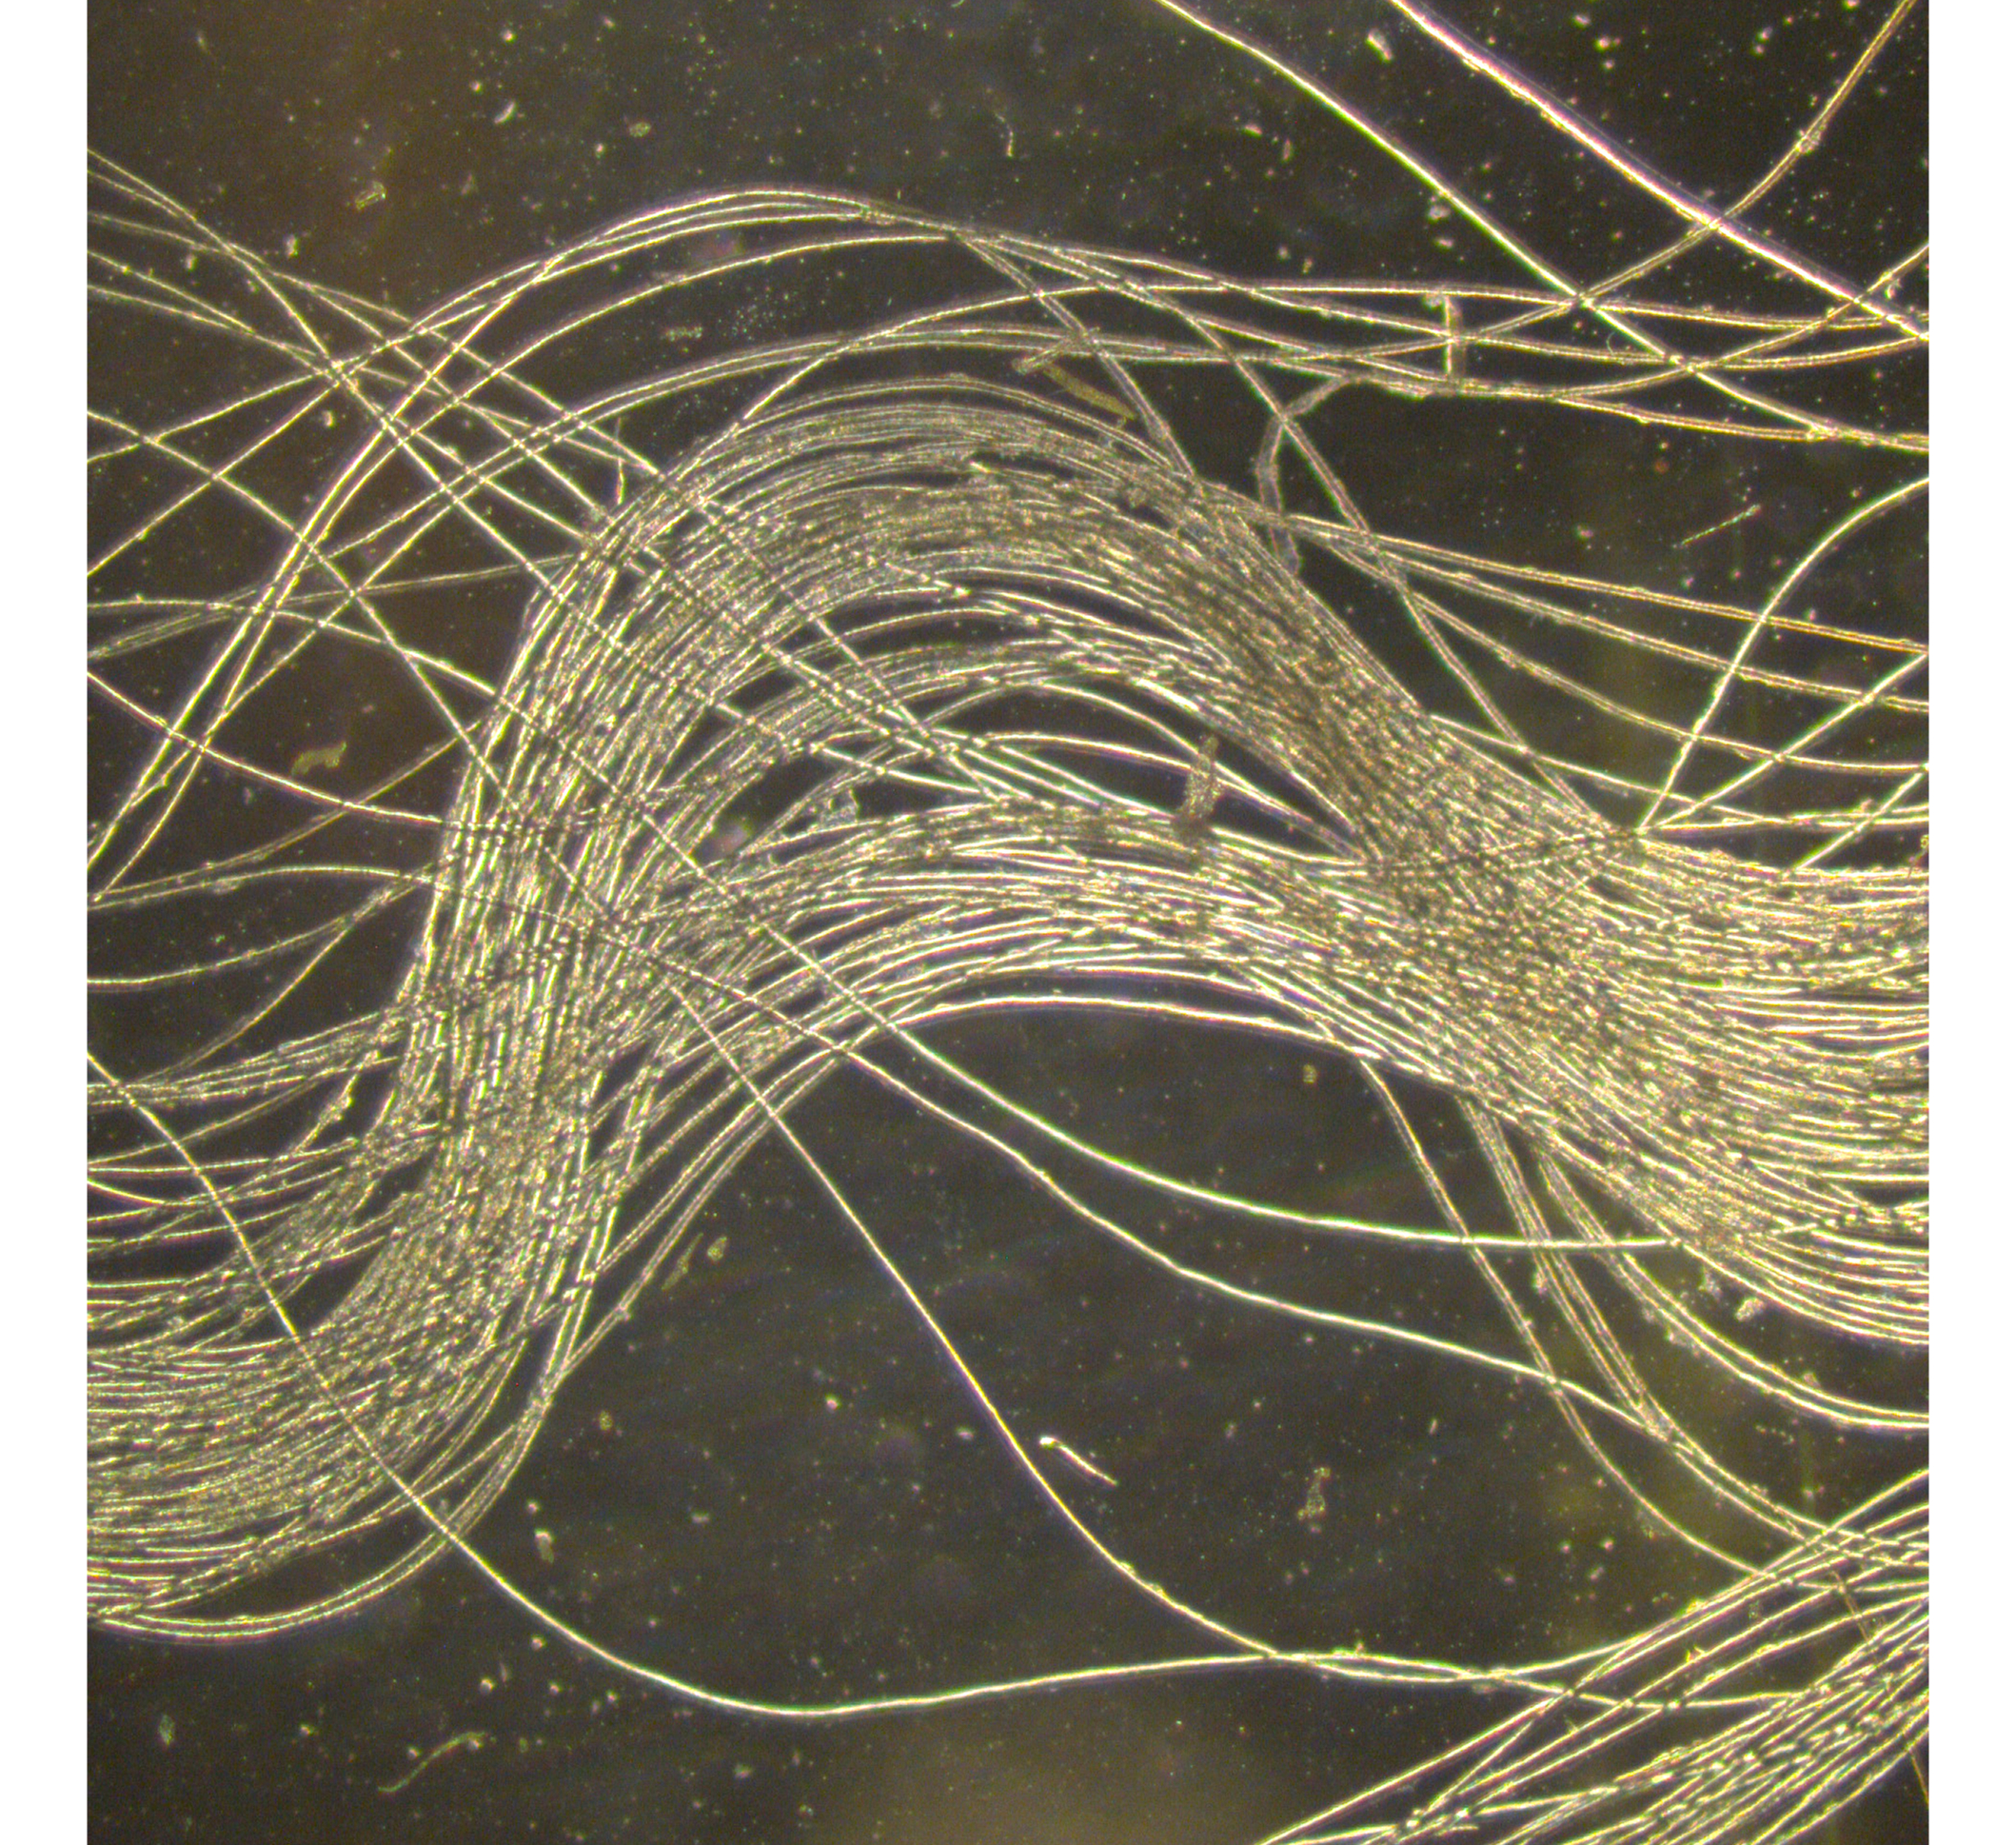
\includegraphics[width=1.0\textwidth]{figtwist.jpg}
  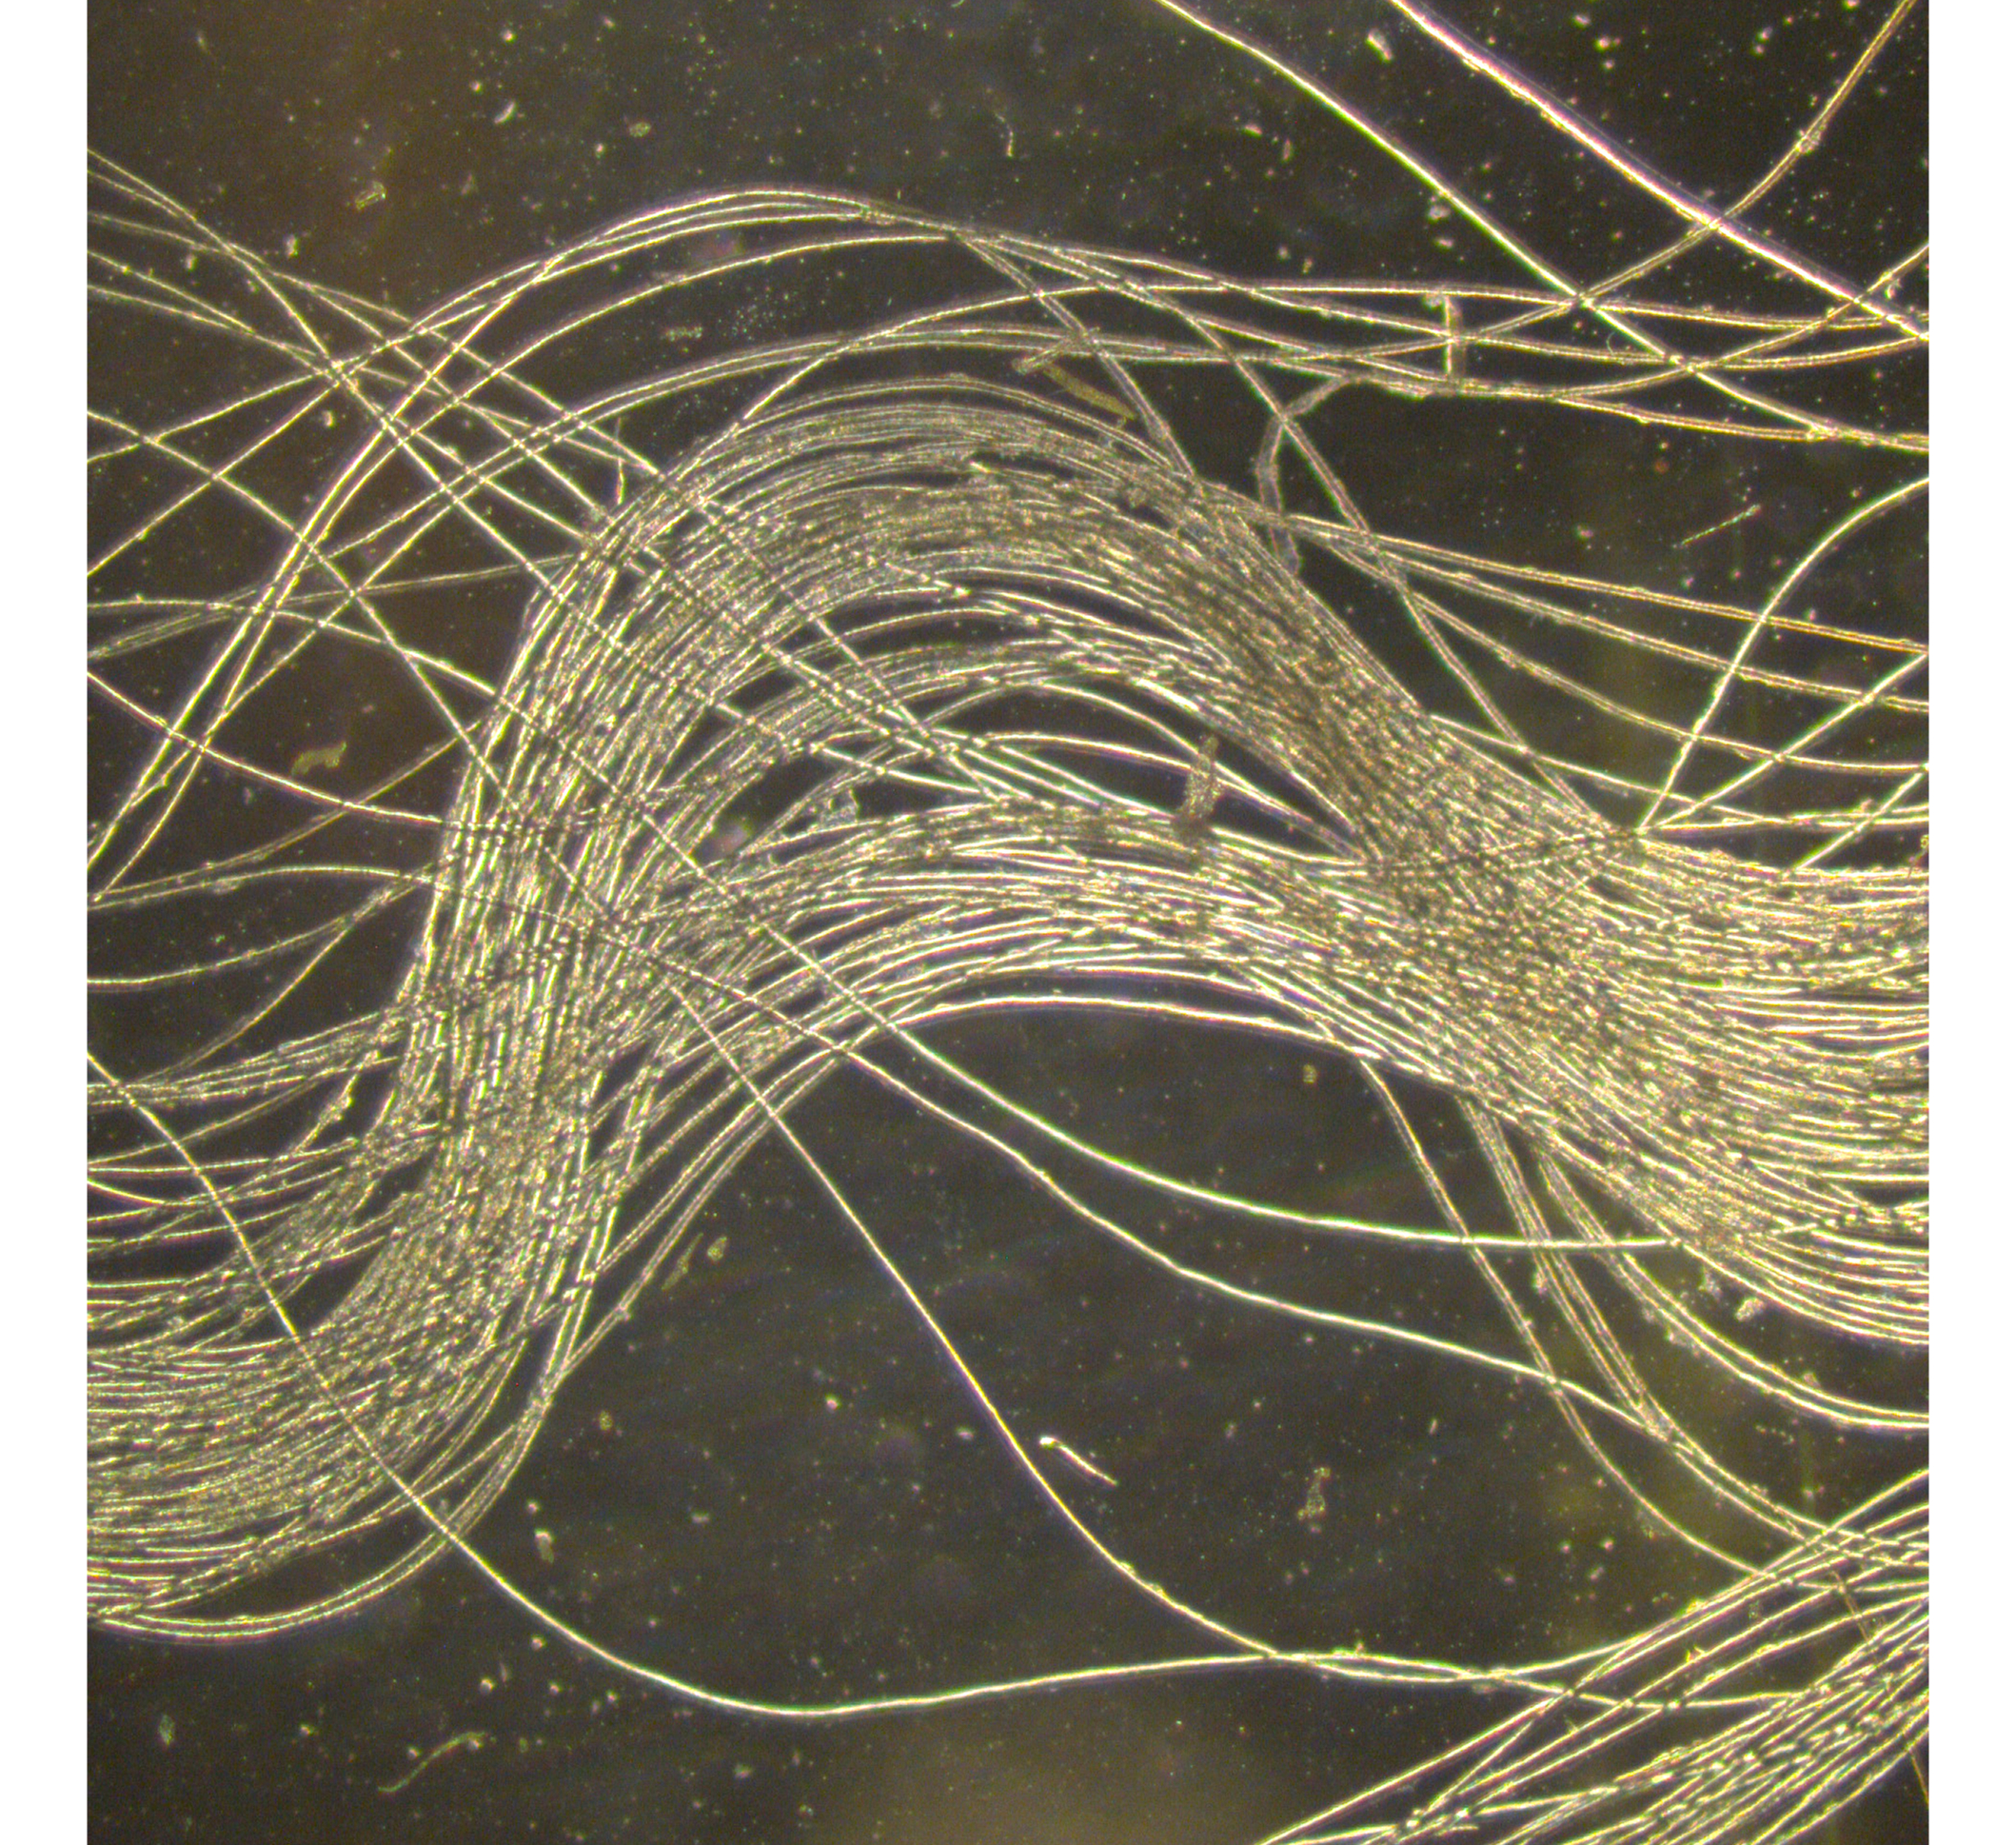
\includegraphics[scale=0.16]{figtwist.jpg}
%   unfo525.jpg is original photo on proj mic
  \caption{Photomicrograph, taken with phase contrast microscope, showing a bundle of fibres from a sheep with semicircular or horseshoe crimp. Note twisted fibres at each of the two points of inflection and absence of twist elsewhere. Note semicircular (non sine wave) shape of the crimp. Microscope magnification 25x. For printed or screen magnification see Appendix }
  \label{fig:twist}
\end{figure}

%\end{document}

